%! Date = 2/23/24

\section{Motivation}\label{sec:motivation}
\begin{table}[!h]
    \centering
    \begin{tabular}{ll}
        \toprule
        \textbf{Notation} & \textbf{Description} \\
        \midrule
        $L$ & Number of layers in $M$ \\
        $i$ & Interval of an MoE layer, $L\equiv 0\:(\mathrm{mod}\: i)$ \\
        $W$ & World Size \\
        $b$ & Micro batch processed in each step  \\
        $s$ & Sequence (or context) length \\
        $h$ & Embedding dimension or hidden size \\
        $k$ & Subset of experts, per token, selected by the Gate \\
        \bottomrule
    \end{tabular}
    \caption{Description of Notation}
    \label{tab:notation}
\end{table}
\begin{figure}[!h]
    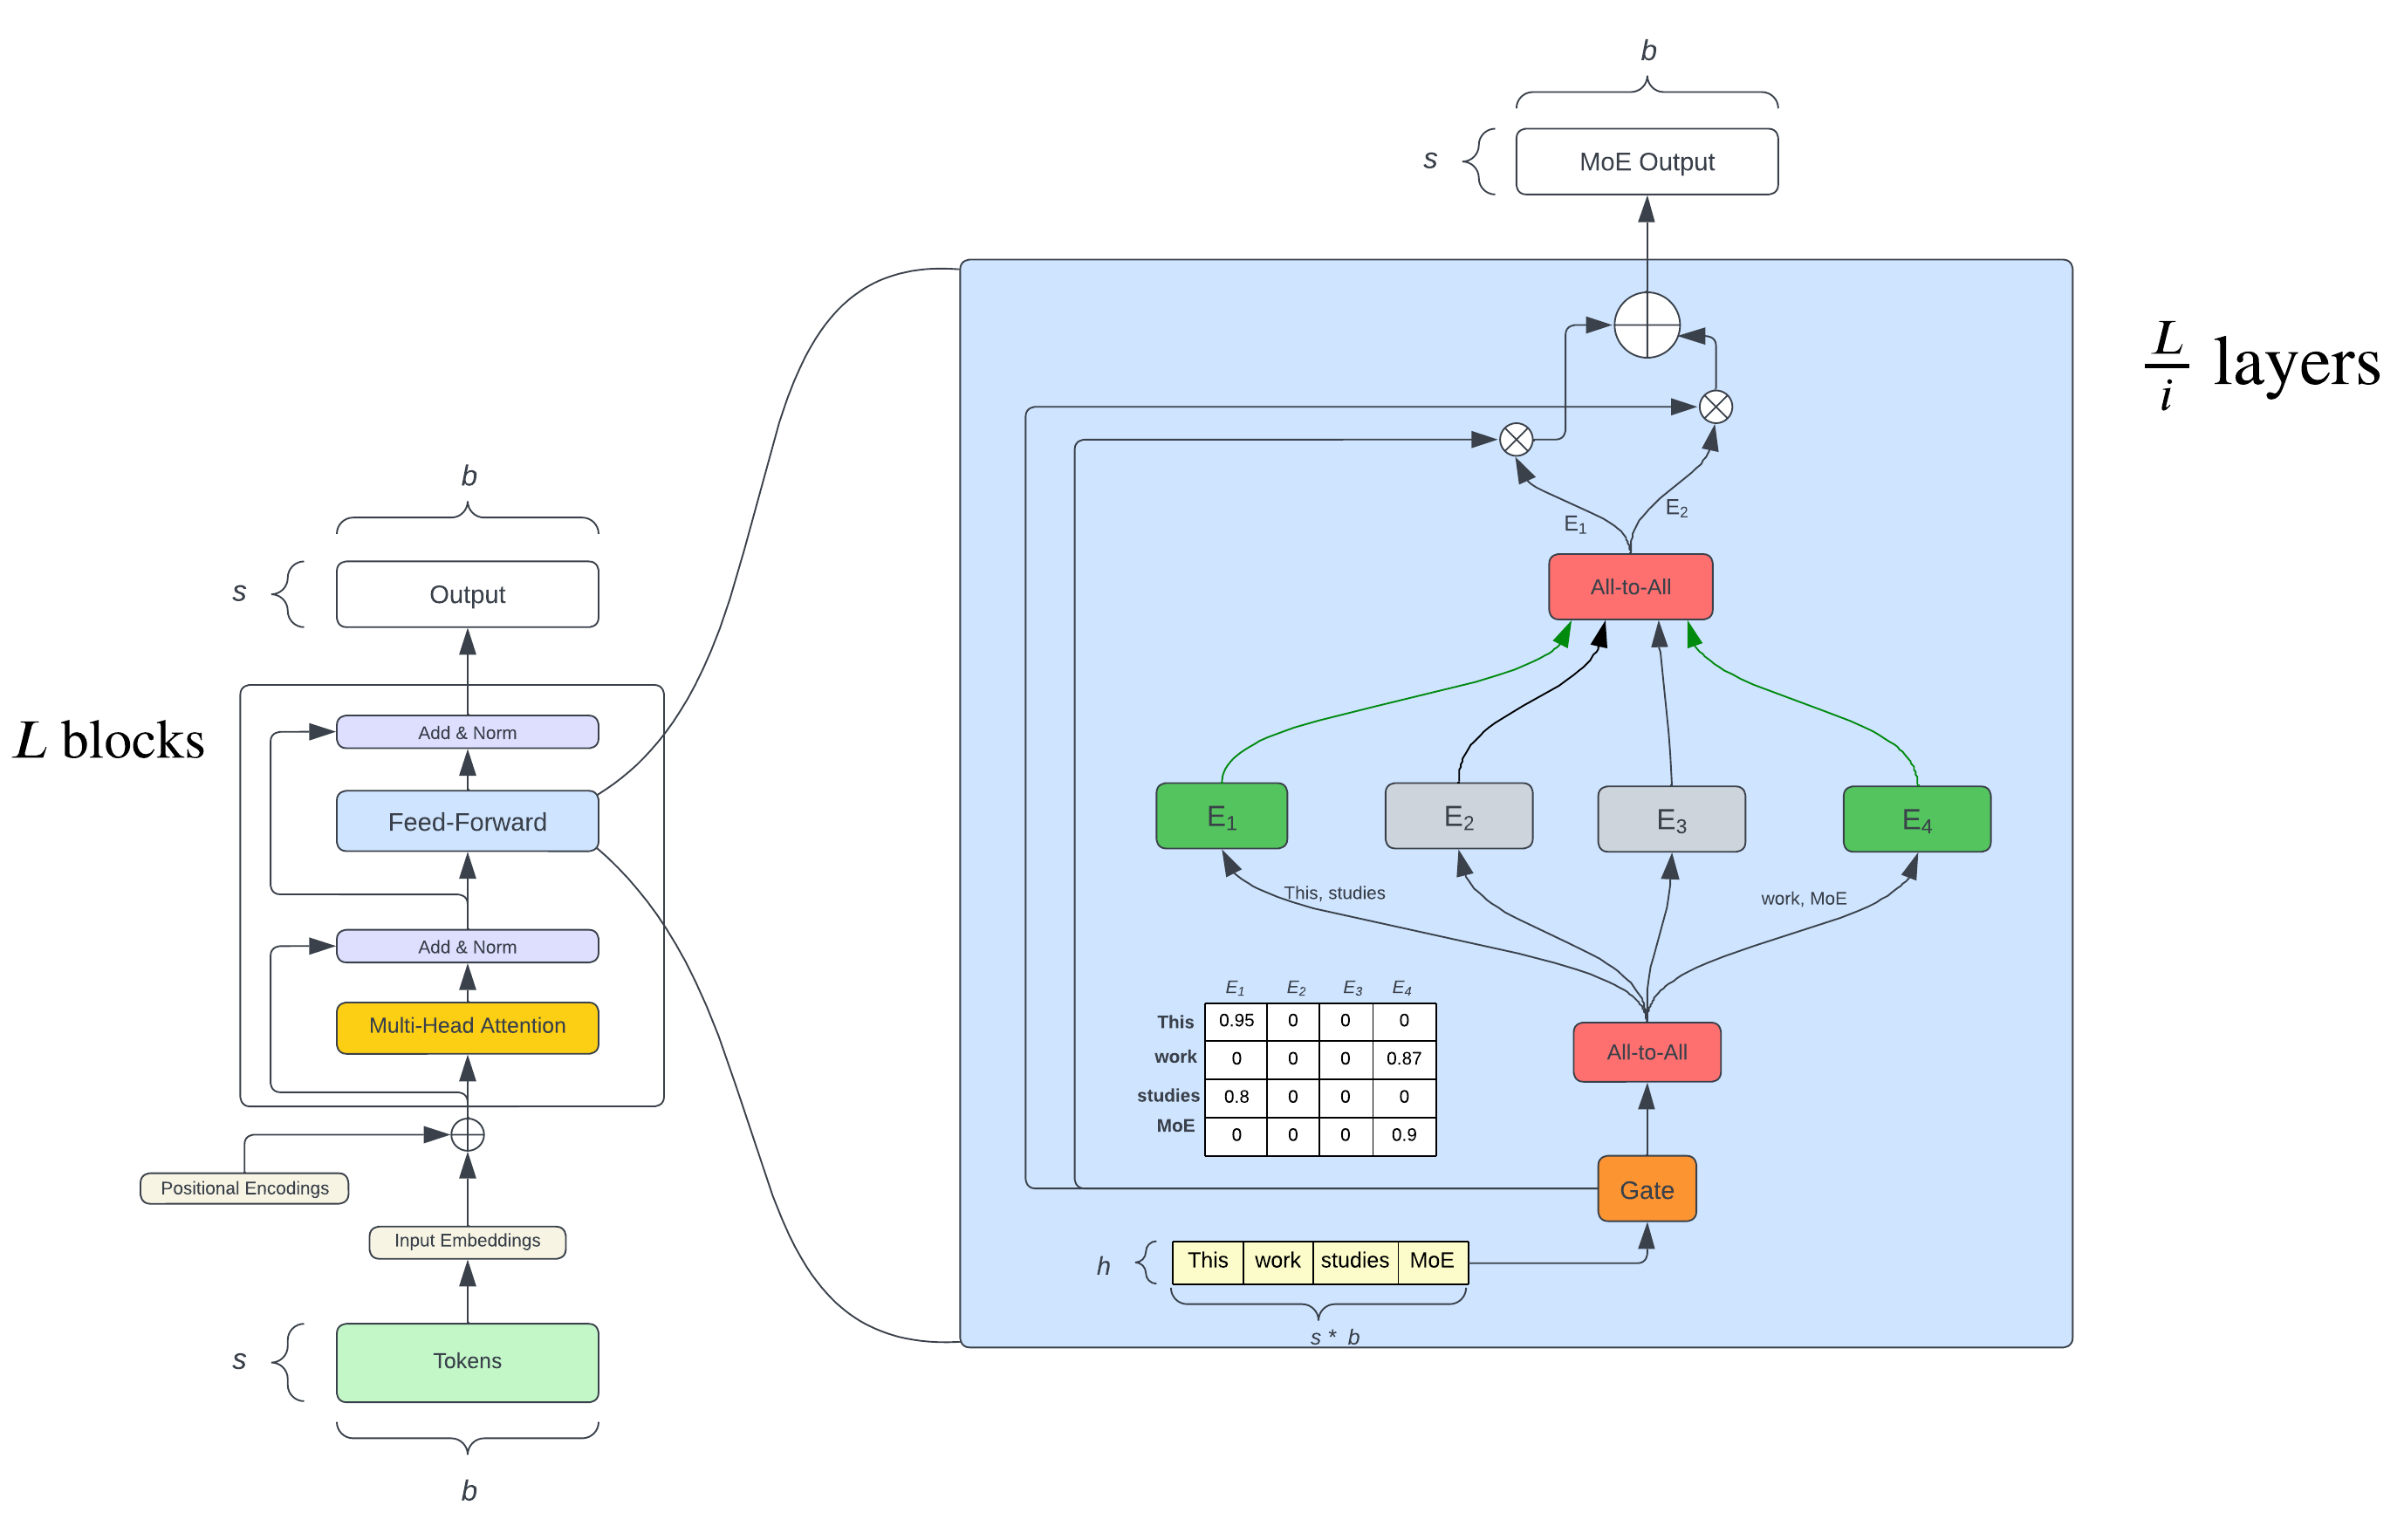
\includegraphics[width=0.75\linewidth]{images/MoE}
    \caption{Distributed MoE Layer as described in~\cite{DBLP:journals/corr/abs-2006-16668}}
    \label{fig:moeLayer}
\end{figure}
Current practice, introduced by Lepikhin et al.,~\cite{DBLP:journals/corr/abs-2006-16668}, for distributed settings
involves sharding the experts and gate networks across workers (GPUs in this work).
Conventional for \emph{expert parallelism} entails each worker hosts $\geq 1$ expert,
such that $W \equiv 0 \: (\mathrm{mod \:}n_E).$.
For example, a sample partitioning for Figure~\ref{fig:moeLayer} could be that each expert $E_j$ resides on a single
worker, yielding $|X|$, the set of all experts.